
%-------------------------------------------------------------------------%
\section{The Standard Model}
The Standard Model (SM) is made up of three generations of spin-$1/2$ \textit{fermions} as fundamental particles, spin-1 \textit{gauge bosons} and the spin-0 \textit{Higgs bosons}. The interactions of the fermionic matter are mediated by the gauge bosons which are modelled well by Quantum Field Theory (QFT); these correspond to the three fundamental forces - electromagnetism, the weak force and the strong force. Unfortunately, the remaining fundamental force, gravity, is yet to be understood at the quantum level. The Higgs, rather the Higgs field, is responsible for the particles acquiring their masses. \\

The fundamental particles comprise of \textit{leptons} and \textit{quarks}, shown in Table \ref{tab:SMFerm}. Each of the three generations of quarks have an up-type and a down-type quark categorized by their electric charges ($+2/3 \text{ or } -1/3$), and the leptons are either charged or neutral, with the neutral components are known as \textit{neutrinos}. The up-type quarks are the \textit{up}, \textit{charm} and \textit{top} quarks, and the down-type quarks are the \textit{down}, \textit{strange} and \textit{bottom} quarks. These quarks exist in a bound state known as \textit{hadrons}, except for the top quark that decay before \textit{hadronisation}, and can never be observed directly. Hadrons are categorized into mesons or (anti-)baryons; Mesons consist of two quarks - a quark-antiquark pair, and (anti-)baryons are made up of three (anti-)quarks. Proton and neutrons are some example of baryons, and pions and kaons are mesons \cite{thomson2013modern}. These fundamental particles differ greatly in mass, with the first generation being the lightest and sequentially becoming heavier for the second and third generations. The first generation of elementary particles represent the basic building blocks of the low energy Universe \cite{thomson2013modern}. \\

\begin{table}[htbp]
    \centering
    \begin{tabular}{c||c|c|c|c}
    \toprule
    & $1^{\text{st}}$ Generation & $2^{\text{nd}}$ Generation & $3^{\text{rd}}$ Generation & Electric Charge \\
    \midrule
    \multirow{2}{1.2cm}{quarks} & $u$ & $c$ & $t$ & $+2/3$ \\
     & $d$ & $s$ & $b$ & $-1/3$ \\
    \midrule
    \multirow{2}{1.2cm}{leptons} & $e$ & $\mu$ & $\tau$ & $\mp1$ \\
     & $\nu_e$ & $\nu_\mu$ & $\nu_\tau$ & $0$ \\
    \bottomrule
    \end{tabular}
    \caption{The symbols of the three generation of spin-$1/2$ fermionic matter in the Standard Model.}
    \label{tab:SMFerm}
\end{table}


The SM is governed by a combination of complex gauge symmetries, $SU_C(3)\times SU_L(2) \times U_\gamma(1)$, with each symmetry described by its corresponding gauge bosons shown in Table \ref{tab:SMBos}. It comprises of four vector bosons in the form of \textit{gluons}, \textit{photons}, \textit{Z bosons} (neutral) and \textit{W bosons} (electrically charged). The gluons mediate the strong force, or strong interactions, described by Quantum Chromodynamics (QCD), binding quarks into hadrons for example. The three remaining gauge bosons are a result of the Higgs mechanism \cite{higgs1964broken, englert1964broken}. The Higgs mechanism involves the Higgs boson, rather the Higgs field - a doublet comprised of a neutral and a charged field component, that acquires some vacuum expectation value (vev). This produces a physical Higgs and three charged and neutral massless Goldstone bosons that are `eaten' by the gauge bosons through electroweak\footnote{The electroweak interaction describes both electromagnetism and the weak interaction as a unified force  ($SU(2)_W \times U(1)_Y$) in the weak scale \cite{thomson2013modern}.} symmetry breaking. The weak gauge bosons $W$ and the $U(1)$ gauge bosons $B$ through the Higgs mechanism provide terms that form the gauge bosons in Table \ref{tab:SMBos}; a mixture of $B$ and $W^0$ that become the massless photon and Z boson that is roughly 91GeV/c$^2$ \cite{tanabashi2018review}, and $W^1 \mp iW^2$ that become the W boson that is roughly 80GeV/c$^2$ \cite{tanabashi2018review}. These terms will be relevant again when we discuss a supersymmetric model. Before considering supersymmetric models, there is an extended theory to the SM known as the Two-Higgs-doublet model (2HDM).  The Higgs sector in the 2HDM has two doublets opposed to the one in SM; the up-type Higgs ($H_u$) and the down-type Higgs ($H_d$) that contain both neutral and charged components. In the 2HDM, the number of degrees of freedom doubles to eight, leading to 5 massless scalar including a SM-like Higgs boson, shown in Table \ref{tab:SMBos}.  \\

\begin{table}[htbp]
    \centering
    {\renewcommand{\arraystretch}{1.2}
    \begin{tabular}{c||c|c}
    \toprule
    Model & Gauge Bosons  & Scalar Bosons \\
    \midrule
    Standard Model & $g$, $\gamma$, $Z^0$, $W^\pm$ & $h^0$ \\
    \hline
    2HDM & $g$, $\gamma$, $Z^0$, $W^\pm$ & $h^0$, $H^0$, $A^0$, $H^\pm$ \\
    \bottomrule
    \end{tabular}}
    \caption{The symbols of the force carriers in the SM and the 2HDM extension.}
    \label{tab:SMBos}
\end{table}


%-------------------------------------------------------------------------%
\subsection{The top quark and its decay}
Amongst the SM particles, the top quarks and their decays will correspond to our background events. The top quark has a rest mass of $m_t\approx175\text{GeV/c}^2$ (we will express mass and energy in natural units $c=1$ hereon) and an electric charge of +2/3$e$ \cite{tanabashi2018review} making it the only known elementary particle in the SM to be heavier than the Higgs boson. The top quark is produced predominantly through gluon-gluon fusion and it almost always decays through the weak interaction into a pair of bottom quark and a W boson. Through the weak interaction, the W boson decays into either a charged lepton-neutrino pair or a pair of quarks and quarks that form hadronic jets. The possible decay modes are given in Figure \ref{fig:topdecay}. \\

%The theoretical predictions of top quarks and the bottom quark was established in 1973 by Kobayashi and Masakawa to explain charge-parity (CP) violation in some meson decays \cite{griffiths2008introduction, kobayashi1973cp}. Experimental evidence for the bottom quark, the generationally paired particle to the top quark, was found at Fermilab in 1977 \cite{herb1977observation}. Nearly two decades later in 1994, the top quark was discovered at the Tevatron with a centre-of-mass energy\footnote{The Centre-of-Mass energy, denoted as $\sqrt{s}$, is a Lorentz invariant value such that $s=\Big( \sum\limits_{i=1}^2 E_i \Big)^2 - \Big( \sum\limits_{i=1}^2 \overrightarrow{p_i} \Big)^2 $. Note that $c=1$ and each $i$ represents the protons in the beam.} of $\sqrt{s}=1.8\text{TeV}$ through the process $p\Bar{p} \rightarrow t\Bar{t}$ \cite{abachi1994search, coll1994evidence, abachi1995observation}. 

\begin{figure}[htbp]
    \centering
    \begin{minipage}{0.24\linewidth}
        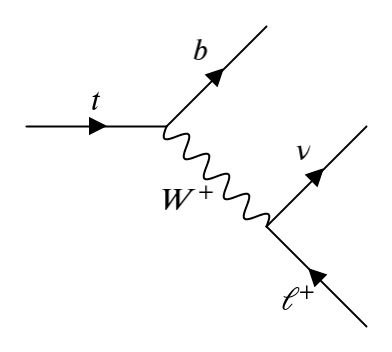
\includegraphics[width=\linewidth]{top1.png}
        \label{fig:top1}
    \end{minipage}
    \begin{minipage}{0.24\linewidth}
        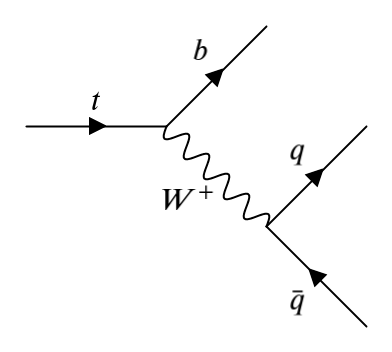
\includegraphics[width=\linewidth]{top2.png}
        \label{fig:anttop1}
    \end{minipage}
    \begin{minipage}{0.24\linewidth}
        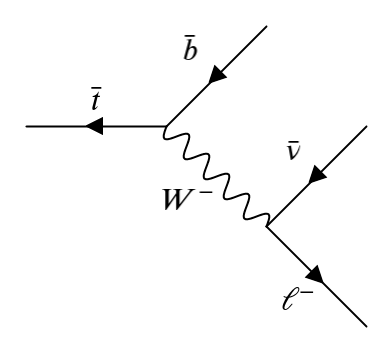
\includegraphics[width=\linewidth]{top3.png}
        \label{fig:top2}
    \end{minipage}
    \begin{minipage}{0.24\linewidth}
        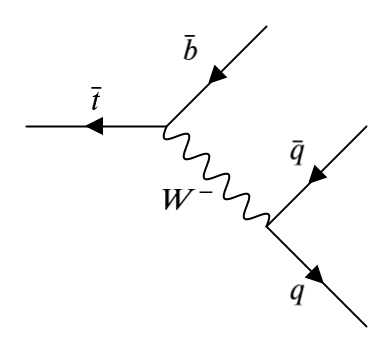
\includegraphics[width=\linewidth]{top4.png}
        \label{fig:anttop2}
    \end{minipage}
    \caption{Feynman diagrams of possible (anti-)top decays. From left to right, we see the top decay with leptonic final states, top decay with hadronic final states, anti-top decay with leptonic final states and anti-top decay with hadronic final states.}
    \label{fig:topdecay}
\end{figure}

%-------------------------------------------------------------------------%
\section{The Minimal Supersymmetric Standard Model}
The Minimal Supersymmetric Standard Model (MSSM) serves as an extension to the SM such that the particle content is duplicated once, thus keeping extra particles introduced to its minimum. Due to the symmetry groups of the SM being contained in the MSSM, any supersymmetric transformation would yield the same quantum numbers as that of the SM \cite{aitchison2007supersymmetry}. The fermions and bosons in the SM shown in Tables \ref{tab:SMFerm} and \ref{tab:SMBos}  have \textit{superpartners}; the supersymmetric counterparts to each particle in the SM as seen in Tables \ref{tab:SUSYspart} and \ref{tab:SUSYinos}. By convention the SM particles and their superpartners are distinguished by a tilde. \\

The superpartners to the SM particles are called \textit{squarks}, \textit{sleptons} and \textit{sneutrinos} whereas the superpartners to the bosons in the SM end with an ``-ino" e.g. \textit{gaugino}. The `symmetry' depicted in supersymmetry is the symmetry between fermions and bosons. This means that the fermions in the SM are bosons in the MSSM and vice versa \cite{martin1997supersymmetry}. Tables \ref{tab:SUSYspart} and \ref{tab:SUSYinos} illustrate that the number of new particles introduced is kept to a \textit{minimum} \cite{aitchison2007supersymmetry}. There is one problem, however. This symmetry we see in Tables \ref{tab:SMFerm}-\ref{tab:SUSYinos} would require that these MSSM particles have the same masses as their SM counterparts. We know this not to be true simply from such particles not being observed in collider experiments thus far. The symmetry must be broken at some high energy scale in an unknown way, allowing these particles to acquire much heavier masses to their SM counterparts that is unobservable with current collider experiments. \\

\begin{table}[htbp]
    \centering
    \begin{tabular}{c||c|c|c}
    \toprule
    & Gen1 & Gen2 & Gen3 \\
    \midrule
    & \\[-2.7ex]
    \multirow{2}{1.4cm}{squarks} & $\Tilde{u}$ & $\Tilde{c}$ & \small$\Tilde{t}$ \\
     & $\Tilde{d}$ & $\Tilde{s}$ & $\Tilde{b}$ \\
    \midrule
    
    \multirow{2}{1.4cm}{sleptons} & $\Tilde{e}$ & $\Tilde{\mu}$ & $\Tilde{\tau}$ \\
     & $\Tilde{\nu_e}$ & $\Tilde{\nu_\mu}$ & $\Tilde{\nu_\tau}$ \\
    \bottomrule
    \end{tabular}
    \caption{The superpartners to the SM quarks and leptons as squarks and sleptons. From the top row, left to right, we have the sup, charm, stop, sdown, sstrange and sbottom quarks, followed by the selectron, smuon and stau for the charged sleptons and their associated sneutrinos as neutral sleptons. As these are bosons, they are now integer spin, namely spin-0 scalar particles.}
    \label{tab:SUSYspart}
\end{table}

\begin{table}[htbp]
    \centering
    \begin{tabular}{c|c}
    \toprule
       Gauginos  & Higgsinos \\
       \midrule
        & \\[-2.5ex]
      $\Tilde{g}$, $\Tilde{B}$, $\Tilde{W}^0$, $\Tilde{W}^\pm$ & $\Tilde{H}_u$,  $\Tilde{H}_d$ \\
     \bottomrule
    \end{tabular}
    \caption{The superpartners to the SM force carriers as gauginos and Higgsinos. The gauginos consist of the gluino, Bino, and Winos (neutral and charged), and the Higgsinos is a superpartner to the 2HDM Higgs with three neutral components ($\Tilde{h}^0$, $\Tilde{H}^0$ and $\Tilde{A}^0$) and two charged components ($\Tilde{H}^\pm$).}
    \label{tab:SUSYinos}
\end{table}

Further expanding on the particles in Table \ref{tab:SUSYinos}, the MSSM introduces dark matter candidates known as \textit{neutralinos}  and \textit{charginos}. These particles are formed as a mixture of the neutral ($\Tilde{H}^0$, $\Tilde{h}^0$, $ \Tilde{A}^0 $, $\Tilde{B}$ and $\Tilde{W}^0$) and charged components ($\Tilde{W}^\pm$ and $\Tilde{H}^\pm$) of the MSSM fermions (excluding the gluino) as shown in Figure \ref{fig:SUSY}. The four neutralinos denoted $\Tilde{\chi}_i^0$ where $i=1,2,3,4$ has four candidates with a mass hierarchy of $ m_{\Tilde{\chi}_1^0} < m_{\Tilde{\chi}_2^0} < m_{\Tilde{\chi}_3^0} < m_{\Tilde{\chi}_4^0}$ \cite{martin1997supersymmetry}. The lightest of the four, $\Tilde{\chi}_1^0$, is thought to be the lightest supersymmetric particle (LSP) which is absolutely stable, supporting the theoretical properties of a proposed dark matter in cosmology. This assumption holds only when \textit{R-parity}, a new form of fundamental symmetry in the MSSM discussed below, is conserved \cite{martin1997supersymmetry}. As $\Tilde{\chi}_i^0$) is the only neutralino that cannot decay, other heavier neutralinos may decay via, but not limited to, two-body decays. In collider experiments, the `detection' of these neutralinos rely on the missing energy of reconstructed SUSY event, much like the SM neutrinos. \\

\begin{figure}[htbp]
    \centering
    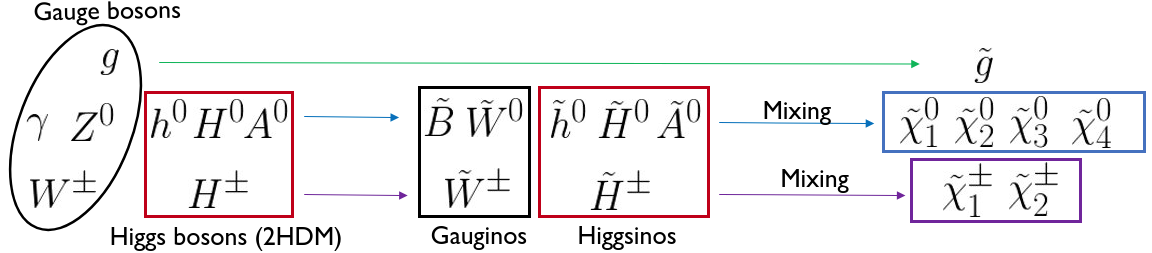
\includegraphics[width=\linewidth]{SUSY.png}
    \caption{Diagram depicting SM force carriers to their MSSM counterparts. The gluon is directly symmetric to the gluino, Higgs bosons and the W boson to the Higgsinos and the charged Winos, respectively. The photon and Z boson are technically part of the $B$ and the $W^3$, thus are symmetric to the Bino and neutral Wino, respectively. The neutral components of the gauginos and Higgsinos mix to give rise to the neutralinos, likewise for the charged components to the charginos.}
    \label{fig:SUSY}
\end{figure}

The new global symmetry \textit{R-parity} is required due to the the quantum numbers known as baryon ($B$) and lepton ($L$) numbers in the SM not considered as fundamental symmetries. This statement is supported by $B$- and $L$- violating processes that are strongly constrained by experiment. R-parity is a conserved quantum number given by Equation (\ref{eq:MPrec})
\begin{equation}
    P_R=(-1)^{3(B-L)+2s}
    \label{eq:MPrec}
\end{equation}
where $s$ is the spin of the particle. This symmetry conveniently separates SM particles and sparticles in a way that the SM particles have $P_R=+1$ (even R-parity), whereas the sparticles all have $P_R=-1$ (odd R-parity) \cite{martin1997supersymmetry}. In MSSM, the conservation of $R$-parity comes from SUSY events as a pair-produced event \cite{aitchison2007supersymmetry}. \\

%\footnote{The gauge invariance required in the SM ``accidentally" \cite{martin1997supersymmetry} guarantees the conservation of such quantum numbers in most interactions.}